\documentclass{article}
\usepackage{geometry}
\usepackage{flafter}
\geometry{letterpaper, portrait, margin=1in}

\usepackage{hyperref}
\hypersetup{
    colorlinks=true,
    linkcolor=black,
    filecolor=magenta,
    urlcolor=blue,
}

\usepackage{graphicx}
\graphicspath{ {images/} }

\usepackage{tcolorbox}
\usepackage{amsmath}
\usepackage{textcomp}
\usepackage{gensymb}
\usepackage{indentfirst}

\newcommand{\ans}{$\rule{1.5cm}{0.15mm}$}

\title{RoboJackets Electrical Training Week 0 Info Sheet}
\author{Alex Xu \\ Joe Spall}
\date{\today\\v1.1}

\begin{document}
\maketitle{}
\setcounter{tocdepth}{2}
\tableofcontents
\vspace{120pt}
\large{Concepts are \textbf{not} necessarily explained in the most physically accurate way. They've been approximated to the level we need. There are many resources online that teach circuits. If the instructors, classmates, or this informational sheet do not explain the topic well enough for you to understand, simply look up the topic and read around.}

\pagebreak

\section{Intro to Electricity}
\subsection{Voltage}

Voltage is the driving force for most, if not all, electrical applications. When people mention voltage, typically they are referring to \textbf{electric field potential difference}. Charged particles naturally move from higher potential to lower potential if there are no other barriers. The value of voltage does not necessarily matter: current may flow from 5V to 3.3V and also from -5V to -12V. \textbf{Charged particles always tend to move if there is a potential difference in place}.

\begin{figure}[!h]
	\center
	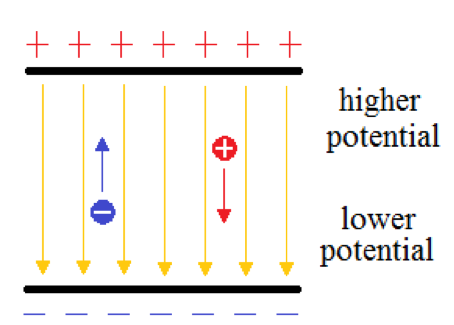
\includegraphics[width=0.3\textwidth, keepaspectratio]{efield}
	\caption{Demo of electric field and potential}
	\label{fig:efield}
\end{figure}

Voltage is measured by a voltmeter. When measuring the voltage across a component, the voltmeter needs to be placed in parallel with the component, since voltage levels are the same across parallel components. To ensure accuracy, voltmeter have such high resistance that it is close to an open circuit. 

\subsection{Current}

Net flow of charged particles is called current (I), measured in Ampere (A). Currents are usually \textbf{induced} by voltages, and when there is no voltage, charged particles just move randomly. This means there is not a measurable amount of current. \par
Amperemeter are used to measure current. Amperemeter need to place in series when measuring current since the current along a single wire segment is always the same. To minimize the influence on the measuring circuit, amperemeter have almost zero resistance and are susceptible to short circuit damage. If the amperemeter does not seem to work, it is very likely the internal fuse was blown from too much current and needs to be replaced.

\subsection{Resistance}

Resistance is a measure of the difficulty to pass a current through the conductor and is measured in Ohm($\ohm$). The resistance can be calculated by dividing the voltage (V) over a component by the current (I) through a component. \par

\begin{figure}[!h]
	\center
	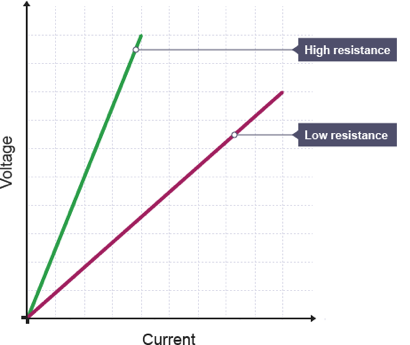
\includegraphics[width=0.35\textwidth, keepaspectratio]{rvi}
	\caption{Example of voltage v. current plot showing resistance.}
	\label{fig:rvi}
\end{figure}

The power (P) dissipated by a resistor is calculated by $V\times I$. This may further expand to $V^2/R$ and $I^2\times R$, since $R=V/I$. In fact, $P=V\times I$ applies to the power dissipation of nearly all electrical components.

\section{Capacitors and Inductors}
\subsection{Capacitors}

A capacitor is a passive two-terminal electrical component that stores potential energy in an electric field. The charging and discharging curves are of exponential feature. The larger the capacitance, the more energy a capacitor can store and the longer it takes to charge / discharge. \par 
Capacitors essentially act as batteries when discharging, so it is useful in dealing with random voltage fluctuations. The electric energy discharged from a capacitor can make up for the temporary drop in supply voltage.

\begin{figure}[!h]
	\center
	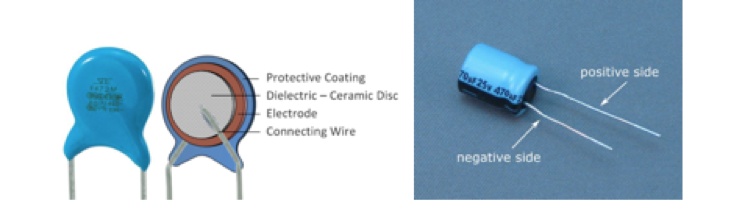
\includegraphics[width=0.6\textwidth, keepaspectratio]{ceramicvelectro}
	\caption{Ceramic (Left) and Electrolytic Capacitor (Right).}
	\label{fig:capacitortype}
\end{figure}

There are primarily two kinds of capacitors: Ceramic and Electrolytic. In our scope of application, we need to know that electrolytics are easy to obtain high capacitance values with low cost but are usually much larger, leading most capacitors on PCBs to be ceramic. Electrolytic capacitors also have polarity.

\subsection{Inductors}

Also known as a coil, an inductor is a passive two-terminal electrical component that stores energy in a magnetic field when current flows through it. \par
Since it is basically a long wire, when exposed to DC, it acts as a wire. Therefore, there is almost zero resistance. \par
On our robots, inductors usually only exist with electro-mechanical parts such as the large emergency stop system on IGVC and RoboRacing robot.

\section{Diodes and FETs}

A diode is a two-terminal electronic component that conducts current primarily in one direction. It has ideally zero resistance in one direction and ideally infinite resistance in the other. Figure \ref{fig:diodeop} is an example of how a diode easily allows forward current and prohibits reverse flow of current. 

\begin{figure}[!h]
	\center
	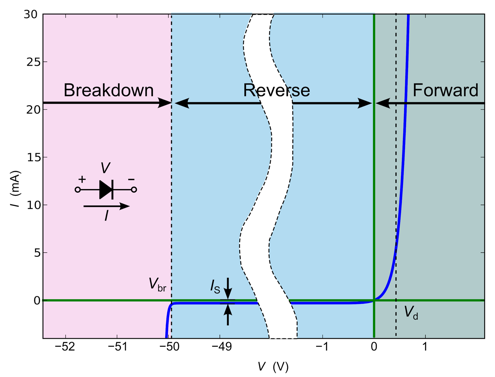
\includegraphics[width=0.35\textwidth, keepaspectratio]{diodeop}
	\caption{Example of diode operation}
	\label{fig:diodeop}
\end{figure}

A light emitting diode (LED) is a special type of diode. When designing a LED circuit, one must consider the maximum current the diode can handle. Figure \ref{fig:LEDcct} is an example of LED circuit. 

\begin{figure}[!h]
	\center
	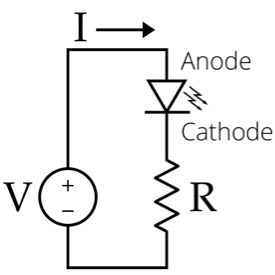
\includegraphics[width=0.3\textwidth, keepaspectratio]{LEDcct}
	\caption{LED Circuit}
	\label{fig:LEDcct}
\end{figure}

Value of R depends on the voltage applied and the type of LED. In most cases, it should be at least larger than voltage divided by suggested current shown in Figure \ref{fig:LEDds} for a common green LED. 

\begin{figure}[!h]
	\center
	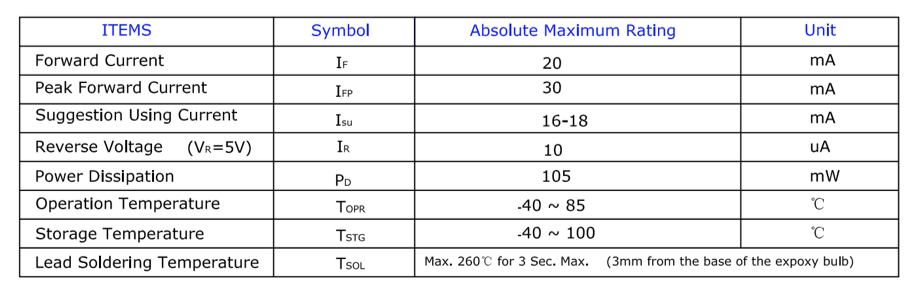
\includegraphics[width=0.7\textwidth, keepaspectratio]{LEDds}
	\caption{LED Datasheet Absolute Maximum Ratings Table}
	\label{fig:LEDds}
\end{figure}

Transistors are simple electronic switches. There are primarily two types of transistors: Bipolar Junction Transistor (BJT) and Metal Oxide Field-Effect Transistor (MOSFET). They typically have 3 terminals, with one acting as the ``controller". There exist two types of BJT: NPN and PNP. NPN is normally OFF and when there's positive voltage at its ``controlling" terminal, NPN conducts current. PNP works in the exact opposite way. \par
MOSFET has nFET and pFET that operates in a similar fashion with NPN and PNP.

\begin{figure}[!h]
	\center
	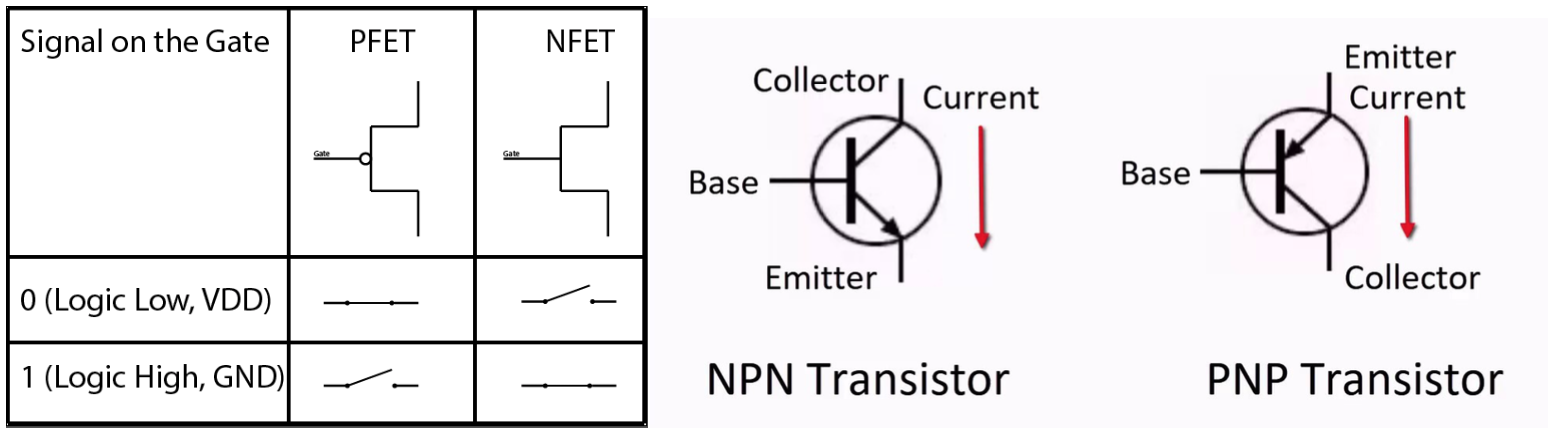
\includegraphics[width=0.7\textwidth, keepaspectratio]{transistor}
	\caption{Sign and operation of MOSFET and BJT.}
	\label{fig:transistor}
\end{figure}

\section{Circuit Analysis}

\textbf{\large{Circuit components in series}}\par

\begin{equation}
\begin{split}
	R_{total} & = \Sigma R_i\\
	C_{total} & = 1/(\Sigma(1/C_i))\\
	L_{total} & = \Sigma L_i
\end{split}
\end{equation}

\textbf{\large{Circuit components in parallel}}\par

\begin{equation}
\begin{split}
	R_{total} & = 1/(\Sigma (1/R_i)\\
	C_{total} & = \Sigma C_i\\
	L_{total} & = 1/(\Sigma (1/L_i)
\end{split}
\end{equation}
\newpage
\textbf{\large{Kirchhoff's Laws}}\par

Kirchhoff's Current Law: Sum of current flowing into a node (or a junction) must be equal to the sum of current flowing out of it. \par
Kirchhoff's Voltage Law: The algebraic sum of the voltage (potential) differences in any closed circuit must equal zero.

\begin{figure}[!h]
	\center
	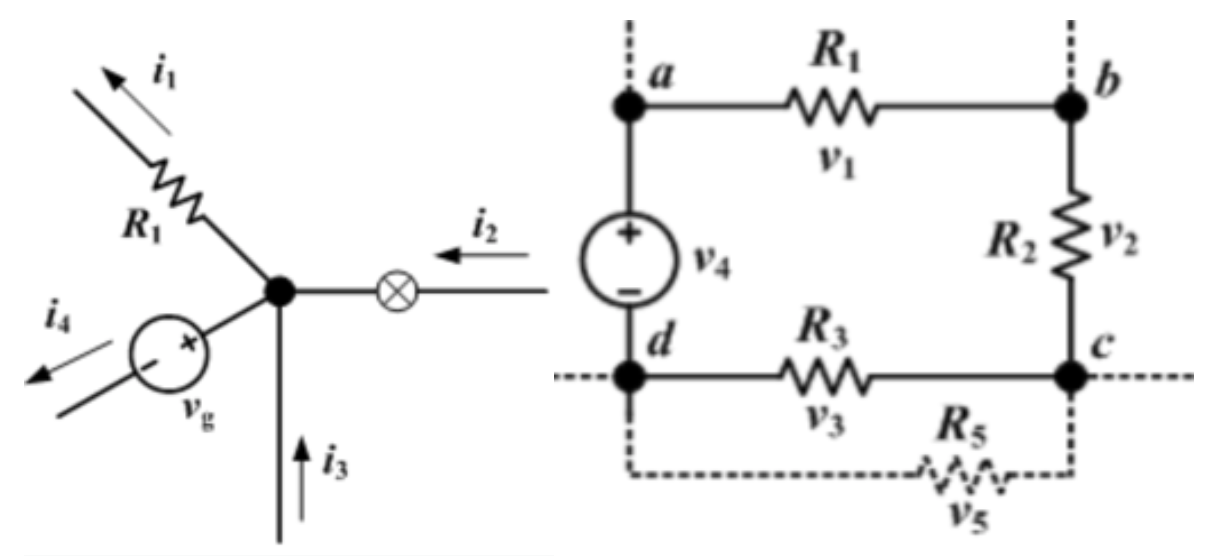
\includegraphics[width=0.5\textwidth, keepaspectratio]{kirchof_demo}
	\caption{Kirchhoff's Law Demonstration}
	\label{fig:kirchof_demo}
\end{figure}
As defined by Kirchhoff's law, in the left diagram $i_2+i_3=i_1+i_4$; in the right figure, $v_1+v_2+v_3+v_4=0$

\section{Application}

Different wire types are better in different instances. Single or solid core is better for breadboarding because it inserts and stays in the holes better. Single-core is usually less flexible and maintains the shape it is bent. Multi-core wire is harder to use when breadboarding and is also much more flexible. \par

Pull-up and pull-down resistors are needed because it helps eliminate high-impedance in signals. Take the following circuit as example: when BUTTON is closed, input\_pin would receive a clear ground signal. However, if R1 and VCC does not exist, and BUTTON is open, input\_pin would receive a floating signal, which could be anywhere between GND and VCC. This creates uncertainty in the signal. Introducing VCC would stabilize the signal to VCC when BUTTON is open, but shorting power to ground when BUTTON is closed. The addition of R1 (in this case a pull-up resistor) solves the shorting issue.

\begin{figure}[!h]
	\center
	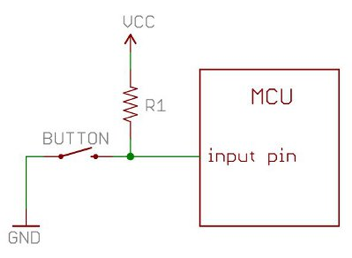
\includegraphics[width=0.3\textwidth, keepaspectratio]{pull}
	\caption{Sample Pull resistor network.}
	\label{fig:pull}
\end{figure}

Blown fuses alert you that there's excessive current, implying either 1. something is broken or 2. redesign the circuit so that the current does not exceed the maximum rating of some components.

\end{document}